\chapter{Implementation} \label{implementation}

For my first implementation attempt, I decided to use the Java programming
language. I chose Java because of its extensive standard library, advanced
parallel processing facilities and my existing familiarity with it. Due to
these factors I was able to quickly iterate on the programs architecture and
data structures. After finishing and testing a simple lexer and parser, I
found that the performance of the program was very dissatisfactory. Optimizing
its performance would have required a deep understanding of the Java virtual
machine. The amount of additional effort required to achieve satisfactory
performance was substantial and besides the topic of my \gls{fyp}.

I started the project over from scratch using the Rust programming language.
Rust, like Java, has very good parallel programming facilities and an extensive
software ecosystem. The experience I gained from the Java implementation meant I
had a working prototype much sooner than with my first attempt. The performance
of the Rust implementation was orders of magnitude faster, even without any
optimization. I continued implementing the relevant research and, once completed
to a satisfactory degree, I submitted this implementation. The following
sections describe its various aspects in more detail.

\begin{listing}[H]
\begin{minted}[linenos]{text}
fn factorial[n: int] {
    if n == 0 {
        return 1;
    } 

    return (n * factorial(n - 1));
}
\end{minted}
\caption{Factorial in the test language.}
\label{lst:example}
\end{listing}

\begin{listing}[H]
\begin{minted}[linenos]{json}
{
  "a": 100,
  "b": {
    "x": [
      100,
      "a"
    ]
  }
}
\end{minted}
\caption{Example of parsable JSON.}
\hrulefill
\label{lst:example}
\end{listing}

Section \ref{dependancies}
\newline \newline
Section \ref{structure}
\newline \newline
Section \ref{outputs_and_visualizations}
\newline \newline
Section \ref{debugging}

\section{Dependencies} \label{dependancies}
\section{Structure} \label{structure}
\subsection{Parsing Grammar Transformation} \label{parsing_grammar_transformation}
\section{Outputs and Visualizations} \label{outputs_and_visualizations}

\begin{figure}[t]
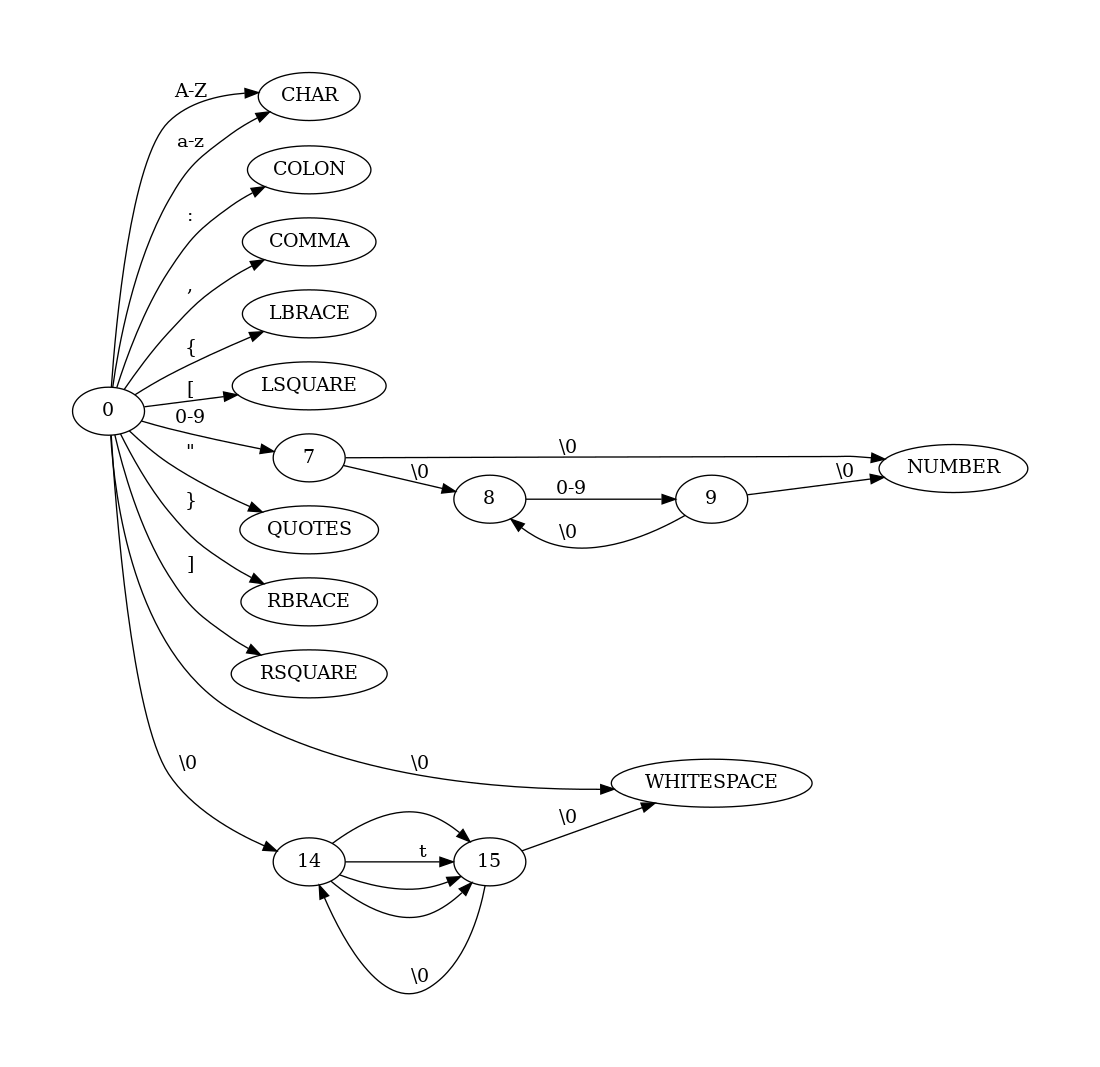
\includegraphics[width=\linewidth]{images/nfa.png}
\caption{NFA of the lexical grammar}
\label{fig:compiler}
\end{figure}

\begin{figure}[t]
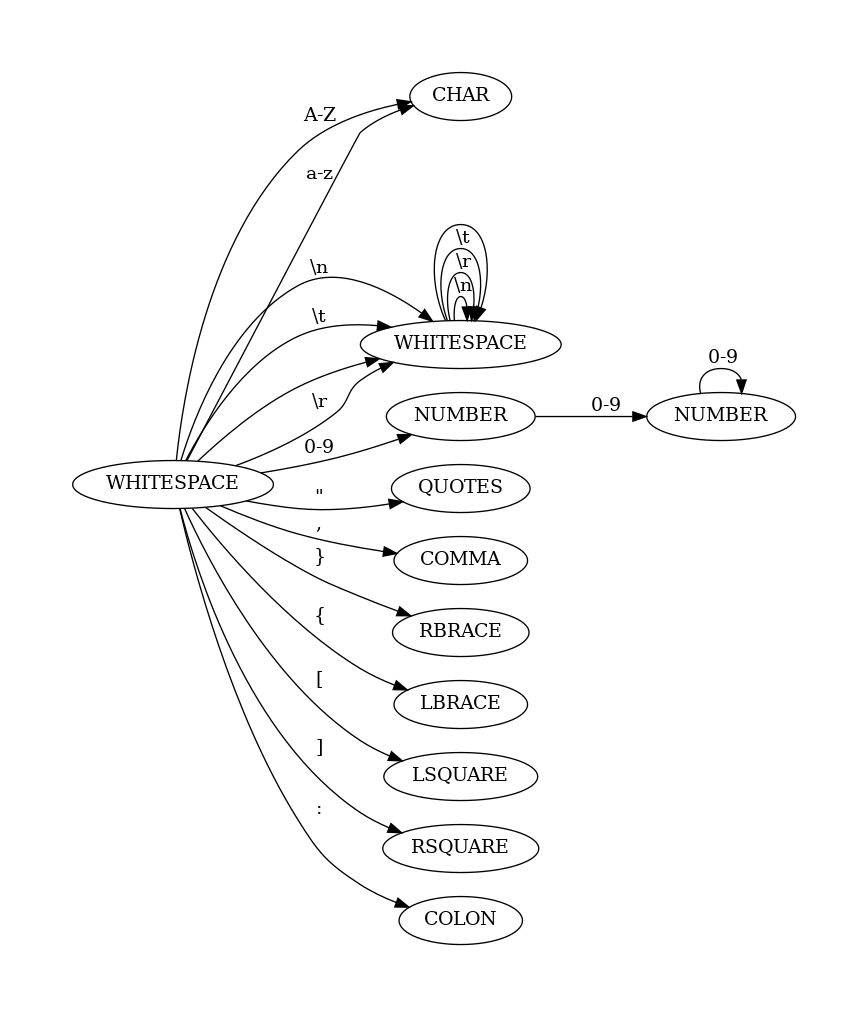
\includegraphics[width=\linewidth]{images/dfa.png}
\caption{DFA of the lexical grammar}
\label{fig:compiler}
\end{figure}

\begin{figure}[t]
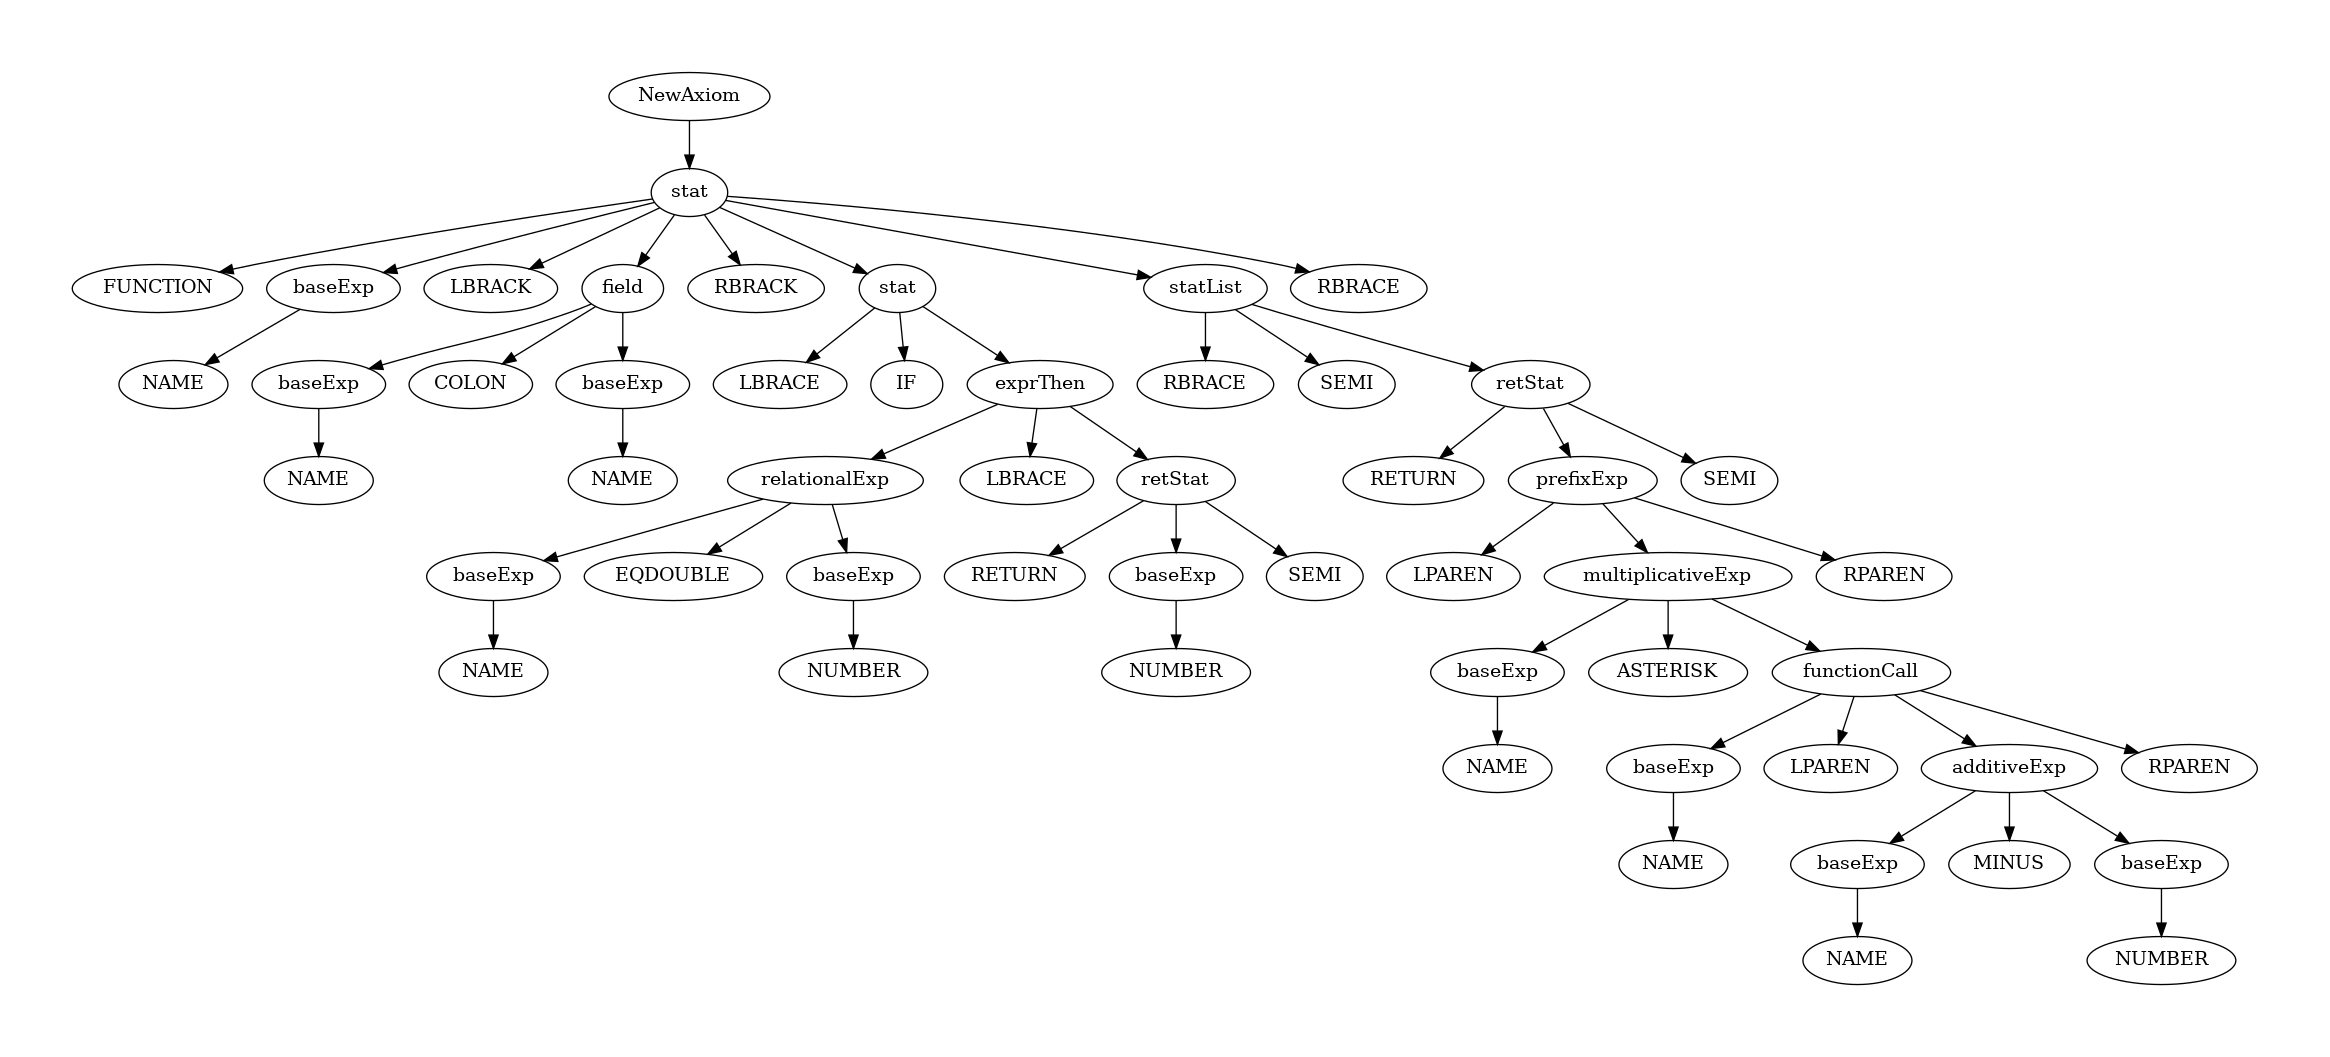
\includegraphics[width=\linewidth]{images/ptree.png}
\caption{Graphviz visualization of the parse tree.}
\label{fig:compiler}
\end{figure}

\section{Debugging} \label{debugging}
